\chapter{Desenvolvimento}

Esta seção tem por propósito apresentar o estudo realizado sobre a
\textit{startup} Rua Dois Tecnologias, sendo esta o objeto de análise
central do presente trabalho. O escopo deste capítulo abrangerá desde
o entendimento sobre o contexto da empresa e sua proposta de valor
até aspectos mais técnicos como a arquitetura do sistema atual e
problemas que já são enfrentados pela \textit{startup} nessa arquitetura.

  As seções estão dispostas em:

  \begin{description}
    \item[Rua Dois Tecnologias:] breve apresentação sobre a empresa e os
      serviços que esta oferece.
    \item[Arquitetura do sistema:] descrição da arquitetura de software atual
      adotada dentro da Rua Dois, e possíveis soluções discutidas dentro da
      empresa a respeito da escalabilidade.
  \end{description}

\section{Rua Dois Tecnologias}

No artigo \textit{Modernizing Real Estate: The Property Tech Opportunity}
\footnote{\url{https://www.forbes.com/sites/valleyvoices/2019/02/22/the-proptech-opportunity}},
a autora \citeonline{LouisaXu} aborda uma visão histórica sobre o desenvolvimento
de tecnologias para o mercado imobiliário fazendo um comparativo com a realidade atual.
Nesse histórico de desenvolvimento, ela relata que desde 1980 são empregados
diversos esforços na área buscando melhorarias por meio de software, mas mesmo
assim, continuamos em uma ramo altamente burocrático e carente de melhorias.

Ciente dessas limitações, PAULO SOBRENOME fundou em outubro de 2018 a
Rua Dois Tecnologias, com o propósito de solucionar as dificuldades
enfrentadas tanto por parte das imobiliárias quanto por parte dos locatários
\footnote{Aquele que mora em um imóvel que não lhe pertence, mediante um
contrato de locação.} no processo de locação de imóveis.

CONVERSAR COM O ERLAN PARA MELHORAR ESSA PARTE

% TODO Conversar com o Erlan para melhorar essa parte
% TODO Explicar o que é CEO e colocar nas lista de abreviações
% TODO Verificar com a Fernanda se tudo bem incluir o nome dela no TCC

\subsection{Serviços prestados}

Visando o processo de locação de imóveis, a Rua Dois conta com quatro serviços
sendo desenvolvidos dentro da empresa, afim de agregar valor aos seus clientes,
sendo eles:

  \begin{enumerate}
    \item \textbf{Captação de Imóveis:} serviço destinado à atrair proprietários de
      imóveis que desejam divulgar o imóvel para locação.
    \item \textbf{Visitas:} serviço de visitas aos imóveis, no qual os interessados em
      locar o imóvel agendam um horário para conhecer o mesmo.
    \item \textbf{Propostas:} serviço no qual os interessados, após passarem pela etapa
      de visitação, avaliam o imóvel e fazem uma proposta para o proprietário do
      imóvel referente ao valor a ser pago pela locação e possíveis ajustes que
      desejam que sejam feitos na propriedade.
    \item \textbf{Contrato:} etapa final, destinada a automatizar a avaliação por parte
      das seguradoras, envio de documentos e assinatura do contrato.
  \end{enumerate}

Cada serviço é vendido de forma separada para as imobiliárias, de forma que cada uma
adapte ao seu contexto os serviços que melhor se encaixam. Atualmente, o serviço
mais desenvolvido é o de visitas e a equipe vem trabalhando com o intuito de
estabilizar os demais serviços.

\section{Arquitetura do sistema}

A arquitetura atual do sistema é composta por dois sistemas principais -
\textit{r2service} e \textit{r2visit}, responsáveis por gerir a maior parte
das funcionalidades relacionadas aos serviços de visitas, propostas, e contrato -
e uma série de sistemas auxiliares e outros serviços que auxiliam no ciclo de
vida do produto. A Figura \ref{fig:ArquiteturaAtual} visa ilustrar esse sistema,
o qual será descrito a seguir conforme está enumerado na figura:


\begin{figure}[h]
  \centering
  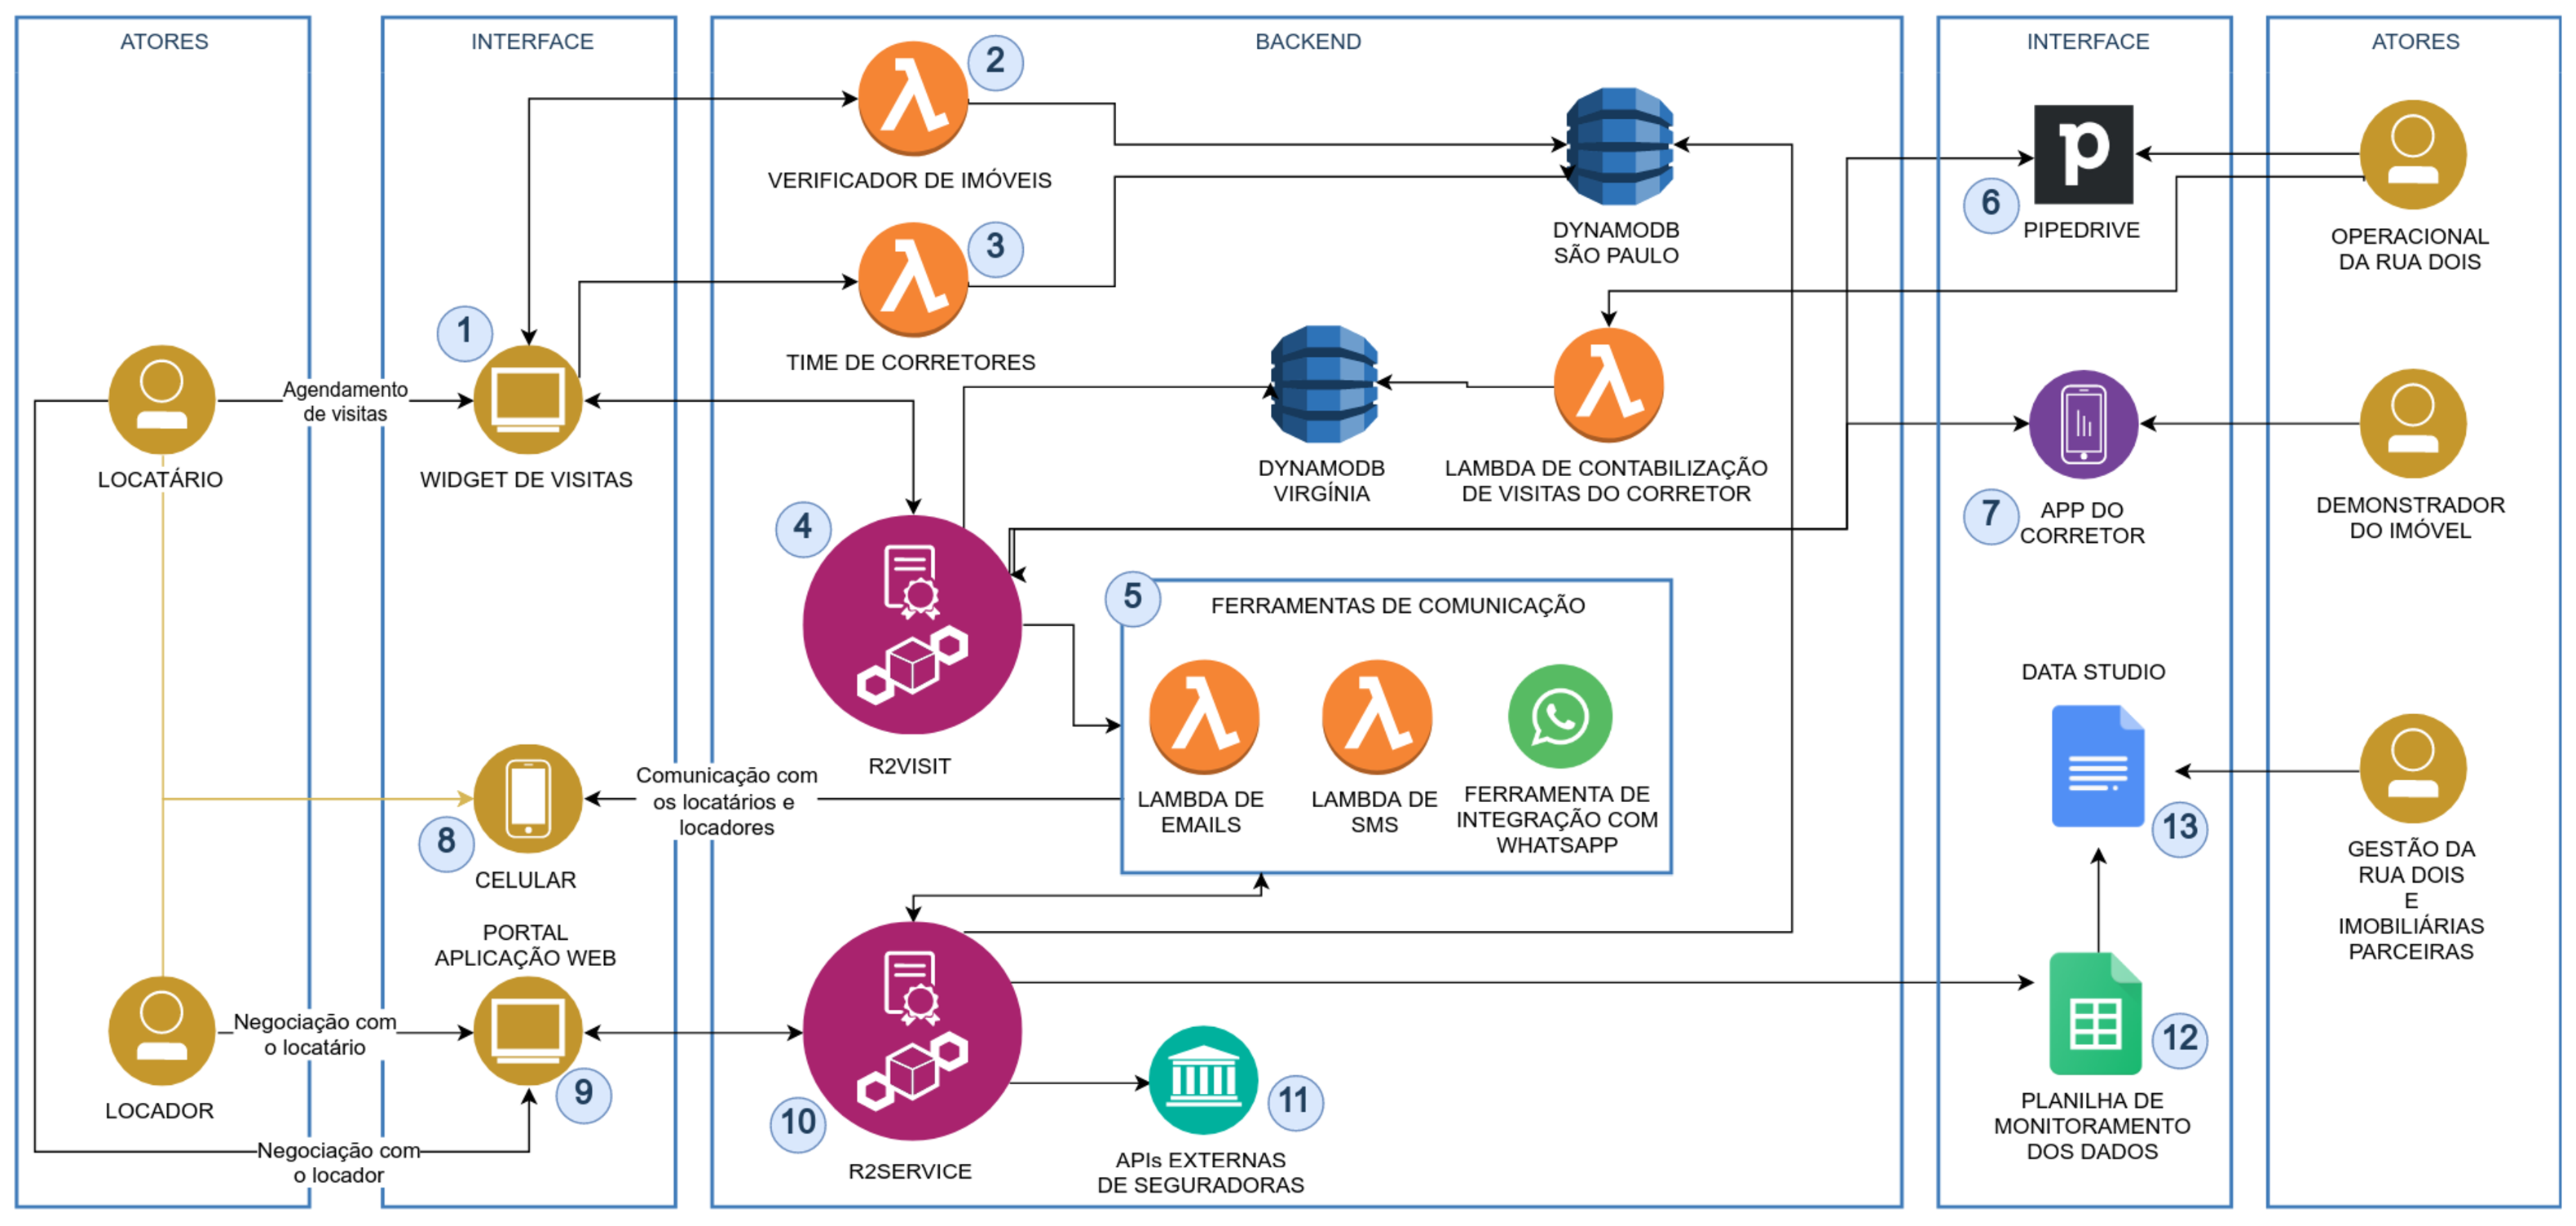
\includegraphics[keepaspectratio=true,scale=0.38]{figuras/r2ArquiteturaAtual.eps}
  \caption{Arquitetura atual do sistema da Rua Dois}
  \label{fig:ArquiteturaAtual}
\end{figure}

  \begin{enumerate}
    \item O \textit{Widget} é um componente utilizado pela Rua Dois que roda no
      \textit{frontend} dos sites das imobiliárias que aderem ao serviço
      de visitas. Ele se comunica com um lambda responsável por verificar se o
      imóvel apresentado no site está disponível no banco de dados da Rua Dois.
      Uma vez que esteja disponível, o \textit{widget} exibe um botão que
      disponibiliza o agendamento da visita \textit{online} para o interessado.
  \end{enumerate}


